\documentclass[border=6pt]{standalone}
\usepackage[T1]{fontenc}
\usepackage[utf8]{inputenc}
\usepackage[scaled=0.98]{helvet}
\renewcommand{\familydefault}{\sfdefault}
\usepackage{amsmath}
\usepackage{graphicx}
\graphicspath{{../../../../../../exercises_lecturenotes/lecture_notes/kurs100_lektionsnoter/}}
\usepackage{tikz}
\usepackage{pgfplots}
\pgfplotsset{compat=1.18}
\usetikzlibrary{arrows.meta, decorations.pathreplacing, calc, positioning, fit, backgrounds, shapes.geometric}
\usepgfplotslibrary{groupplots,fillbetween}
\definecolor{scanpink}{HTML}{E5006D}
\definecolor{scanteal}{HTML}{00A6A6}
\definecolor{scannavy}{HTML}{243746}
\definecolor{scanlightgray}{HTML}{F1F2F3}
\begin{document}
  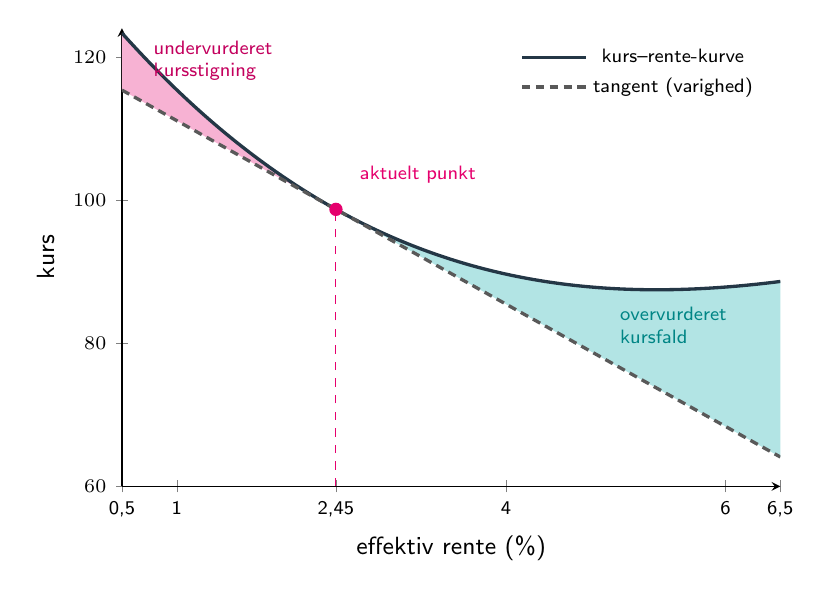
\begin{tikzpicture}

    % Skematisk kursfunktion.
    %
    % Kurven går gennem det aktuelle punkt (2,45 ; 98,696)
    % og har samme tangent som varighedsapproksimationen dér.
    % Konveksiteten er bevidst fremhævet for at gøre forskellen
    % mellem kurskurven og tangenten tydelig i figuren.
    \pgfmathdeclarefunction{kapFourBondPrice}{1}{%
      \pgfmathparse{
        98.696
        - 8.542*(#1-2.45)
        + 1.90*(#1-2.45)^2
        - 0.10*(#1-2.45)^3
      }%
    }

    \begin{axis}[
      width=0.82\textwidth,
      height=7.4cm,
      axis lines=left,
      xlabel={effektiv rente (\%)},
      ylabel={kurs},
      xmin=0.5,
      xmax=6.5,
      ymin=60,
      ymax=124,
      xtick={0.5,1,2.45,4,6,6.5},
      xticklabels={0{,}5,1,2{,}45,4,6,6{,}5},
      ytick={60,80,100,120},
      legend style={
        draw=none,
        fill=none,
        font=\scriptsize,
        at={(0.98,0.98)},
        anchor=north east
      },
      legend image post style={xscale=1.35},
      tick label style={font=\scriptsize},
      label style={font=\small}
    ]

      % -------------------------------------------------
      % Usynlige kurver til definition af de farvede arealer
      % -------------------------------------------------

      \addplot[
        name path=kurskurve,
        draw=none,
        domain=0.5:6.5,
        samples=250,
        forget plot
      ]
        {kapFourBondPrice(x)};

      \addplot[
        name path=varighedstangent,
        draw=none,
        domain=0.5:6.5,
        samples=2,
        forget plot
      ]
        {98.696 - 8.542*(x-2.45)};

      % -------------------------------------------------
      % Rentefald:
      % tangenten undervurderer kursstigningen
      % -------------------------------------------------

      \addplot[
        fill=scanpink!30,
        draw=none,
        forget plot
      ]
        fill between[
          of=kurskurve and varighedstangent,
          soft clip={domain=0.5:2.45}
        ];

      % -------------------------------------------------
      % Rentestigning:
      % tangenten overvurderer kursfaldet
      % -------------------------------------------------

      \addplot[
        fill=scanteal!30,
        draw=none,
        forget plot
      ]
        fill between[
          of=kurskurve and varighedstangent,
          soft clip={domain=2.45:6.5}
        ];

      % -------------------------------------------------
      % Skematisk kurs-rente-kurve
      % -------------------------------------------------

      \addplot[
        scannavy,
        very thick,
        domain=0.5:6.5,
        samples=250,
        forget plot
      ]
        {kapFourBondPrice(x)};

      % Manuel legend, så linjetypen vises korrekt
      \addlegendimage{
        scannavy,
        very thick
      }
      \addlegendentry{kurs--rente-kurve}

      % -------------------------------------------------
      % Tangent bestemt af varigheden
      % -------------------------------------------------

      \addplot[
        black!65,
        very thick,
        dash pattern=on 3pt off 2pt,
        domain=0.5:6.5,
        samples=2,
        forget plot
      ]
        {98.696 - 8.542*(x-2.45)};

      % Manuel legend med tydeligt stiplet linje
      \addlegendimage{
        black!65,
        very thick,
        dash pattern=on 3pt off 2pt
      }
      \addlegendentry{tangent (varighed)}

      % -------------------------------------------------
      % Aktuelt punkt
      % -------------------------------------------------

      \addplot[
        only marks,
        mark=*,
        mark size=2.2pt,
        scanpink,
        forget plot
      ]
        coordinates {(2.45,98.696)};

      \draw[
        scanpink,
        dashed
      ]
        (axis cs:2.45,60)
        --
        (axis cs:2.45,98.696);

      \node[
        font=\scriptsize,
        scanpink,
        anchor=south west
      ] at (axis cs:2.58,101.0) {
        aktuelt punkt
      };

      % -------------------------------------------------
      % Forklarende labels
      % -------------------------------------------------

      \node[
        font=\scriptsize,
        scanpink!85!black,
        align=left,
        anchor=west
      ] at (axis cs:0.70,119.5) {
        undervurderet\\
        kursstigning
      };

      \node[
        font=\scriptsize,
        scanteal!80!black,
        align=left,
        anchor=east
      ] at (axis cs:6.10,82.5) {
        overvurderet\\
        kursfald
      };

    \end{axis}
  \end{tikzpicture}
\end{document}
